%http://www.math.uconn.edu/~kconrad/blurbs/
\documentclass[oneside,a4paper,12pt]{article}
\usepackage[english,brazilian]{babel}
\usepackage[alf]{abntex2cite}
\usepackage[utf8]{inputenc}
\usepackage[T1]{fontenc}
\usepackage[top=20mm, bottom=20mm, left=20mm, right=20mm]{geometry}
\usepackage{framed}
\usepackage{booktabs}
\usepackage{color}
\usepackage{hyperref}
\usepackage{graphicx}
\usepackage{float}
\usepackage{pstricks}
\graphicspath{{./Figuras/}}    
\definecolor{shadecolor}{rgb}{0.8,0.8,0.8}

\usepackage{tikz}
\usepackage[utf8]{inputenc}
\usepackage{mathtext}
\usepackage{graphicx}
\usepackage{verbatim}
\usepackage{wrapfig}
\usepackage[T1]{fontenc}
\usepackage{blindtext}
\usepackage{tasks}
\usepackage{fancybox}
\usepackage{amsthm}
\usepackage{setspace}
\usepackage{amsmath}
\usepackage{amsfonts}
\usepackage{amssymb}
\usepackage{graphicx, color}
\newcommand{\sen}{{\rm sen}}
\newcommand{\tg}{{\rm tg}}
\newcommand{\cotg}{{\rm cotg}}
\newcommand{\cossec}{{\rm cossec}}
\newcommand{\arctg}{{\rm arctg}}
\newcommand{\arcsen}{{\rm arcsen}}
\newcommand{\negrito}[1]{\mbox{\boldmath{$#1$}}} 
\usepackage{pifont}
\usepackage{multicol}
\usepackage[framemethod=TikZ]{mdframed}
\newcommand{\heart}{\ensuremath\heartsuit}
\newcommand{\diamonde}{\ensuremath\diamondsuit}
\theoremstyle{Colorido}
\newtheorem{questao}{\textcolor{Floresta}{\textit{\bf Questão}}}
\newtheoremstyle{Colorido}{}{}{\color{Floresta}}{}{\color{Floresta}\bfseries}{}{ }{}
\newtheorem{theorem}{Theorem}
\newtheoremstyle{solu}{}{}{}{}{\color{red}\bfseries}{}{ }{}
\theoremstyle{solu}
\newtheorem*{resp}{Solução}
\newtheoremstyle{dotlessP}{}{}{}{}{\color{Floresta}\bfseries}{}{ }{}
\theoremstyle{dotlessP}
\newcommand{\solucao}[1]{\textcolor{blue}{\textbf{Solução:} #1}}
\newtheorem{sol}{Questão}
%FAZ EDICOES AQUI (somente no conteudo que esta entre entre as ultimas  chaves de cada linha!!!)
\newcommand{\universidade}{Programa de Iniciação Científica OBMEP}
\newcommand{\centro}{PIC 2020}
%\newcommand{\departamento}{Departamento}
%\newcommand{\curso}{Curso}
\newcommand{\professor}{Douglas de Araujo Smigly}
\newcommand{\disciplina}{Programa de Iniciação Científica}
\newcommand{\entrega}{ }
\DeclareSymbolFont{extraup}{U}{zavm}{m}{n}
\DeclareMathSymbol{\varheart}{\mathalpha}{extraup}{86}
\DeclareMathSymbol{\vardiamond}{\mathalpha}{extraup}{87}
	\cornersize{.3} 
	\mdfdefinestyle{MyFrame}{%
    linecolor=blue,
    outerlinewidth=2pt,
    roundcorner=20pt,
    innertopmargin=\baselineskip,
    innerbottommargin=\baselineskip,
    innerrightmargin=20pt,
    innerleftmargin=20pt,
    backgroundcolor=gray!24!white}
%ATE AQUI !!!

\begin{document}
\definecolor{Floresta}{rgb}{0.13,0.54,0.13}
	\pagestyle{empty}
	
	\begin{center}
	
\includegraphics[width=\linewidth/3]{logo_pic}%LOGOTIPO DA INSTITUICAO
	 	\vspace{0pt}
	 	
		\universidade
		\par
		\centro
		\par
%		\departamento
		\par
%		\curso
		\par
		\vspace{24pt}
		\LARGE \textbf{Avalia\c c\~ao - Ciclo I}
		
	\end{center}
	
	\vspace{24pt}
	
	%
%	\begin{tabular}{ |l|p{12cm}| }
%		
%		\hline
%		\multicolumn{2}{|c|}{\textbf{Dados de Identificação}} \\
%			\hline
%		Disciplina:        &    \disciplina          \\
%		\hline
%		Professor:         &    \professor           \\
%	\hline
%	Aluno(a):         &\\
%		\hline
%	Multiplicidade:  & \ \ \ \ \ \ \vline Nível: \vline\\
%	
%		\hline
	%\end{tabular}
	%
	

	\begin{tabular}{ |l|p{12cm}| }
		
		\hline
		\multicolumn{2}{|c|}{\textbf{Dados de Identificação}} \\
			\hline
		Curso:        &  \disciplina \\
			\hline
		Nome:        &  \\
		\hline
		Nível:      &  \\
		\hline
				Multiplicidade:      &  \\
		\hline
				Assinatura:      &  \\
		\hline
				Data de entrega:      &  \entrega \\
		\hline
	\end{tabular}
	
	\vspace{24pt}
	\vspace{40pt}
	\tableofcontents
	\begin{comment}	
\begin{multicols*}{2}
	\begin{center}
		\begin{tabular}{ |c|p{1.9cm}| }
		
		\hline
		\multicolumn{2}{|c|}{\textbf{Tarefa Online}} \\
			\hline
		\centering\textbf{Questão}        &  \textbf{Resposta}\\
		\hline
		Questão 1        & (b)\\
		\hline
		Questão 2        & (c)\\
		\hline
		Questão 3        & (c)\\
		\hline
		Questão 4        &\\
		\hline
		Questão 5        &\\
		\hline
		Questão 6        &\\
		\hline
		\textbf{Total}        &\\
		\hline
	\end{tabular}
	\end{center}
\columnbreak
		\begin{center}
		\begin{tabular}{ |c|p{1.9cm}| }
		
		\hline
		\multicolumn{2}{|c|}{\textbf{Avaliação Online}} \\
			\hline
		\centering\textbf{Questão}        &  \textbf{Resposta}\\
		\hline
		Questão 1        &\\
		\hline
		Questão 2        &\\
		\hline

		\textbf{Total}        &\\
		\hline
	\end{tabular}
	\end{center}
	
	\end{multicols*}
	\vspace{24pt}
	\end{comment}
	%\begin{snugshade}
	%	\section{O... aumento  }  
	%\end{snugshade}
	\newpage	
	\textcolor{Floresta}{\section{Tarefa Online}}
	\begin{sol}
\textit{(0,5 ponto)} 
Duas cidades $A$ e $B$ são separadas por um rio. Dois tipos de barcos fazem a travessia entre as duas cidades, com velocidades constantes. O barco do tipo I faz a travessia em $20$ minutos e o do tipo II em $15$ minutos. O horário em que o barco do tipo II que saiu da cidade A às $10$ horas e $6$ minutos se encontra com o barco do tipo I que saiu da cidade B às $10$ horas é:
\begin{tasks}[counter-format={(tsk[a])},label-width=3.6ex, label-format = {\bfseries}, column-sep = {20pt}](1)
\task[\textcolor{blue}{$\negrito{(a)} $}] $10$ horas e $8$ minutos.
\task[\textcolor{blue}{$\negrito{(b)} $}] $10$ horas e $12$ minutos.
\task[\textcolor{blue}{$\negrito{(c)} $}] $10$ horas e $16$ minutos.
\task[\textcolor{blue}{$\negrito{(d)} $}] $10$ horas e $20$ minutos.
\task[\textcolor{blue}{$\negrito{(e)} $}] $10$ horas e $24$ minutos.
\end{tasks}
\end{sol}
\textcolor{blue}{\textbf{Solução:}
Sejam $v_I$ e $v_{II}$ as velocidades dos barcos dos tipos I e II, respectivamente. Seja $d$ a distância entre as duas cidades. Então, $v_I=\dfrac{d}{20}$ e $v_{II}=\dfrac{d}{15}$. Seja $t$ minutos o tempo decorrido entre o instante que o barco do tipo I saiu da cidade B e o instante em que os dois barcos se encontram. Como a soma das distâncias percorridas pelos dois barcos até o encontro é igual a $d$, então $v_{II}(t-6)+v_It=d$. Como $v_I=\dfrac{d}{20}$, $v_{II}=\dfrac{d}{15}$ e $v_{II}(t-6)+v_It=d$, então $\dfrac{d}{15}(t-6)+\dfrac{d}{20}t=d$. Dividindo ambos os membros desta última equação por $d$, obtém-se $\dfrac{t-6}{15}+\dfrac{t}{20}=1$. Resolvendo a equação linear $\dfrac{t-6}{15}+\dfrac{t}{20}=1$, obtém-se $t=12$. Assim, o horário do encontro dos dois barcos é $10$ horas e $12$ minutos. A alternativa correta é a alternativa (b).
}
		%\vspace{60pt}
		\newpage	
	\begin{sol}
\textit{(0,5 ponto)} \newline \newline
Pedro é atleta de corrida. Em seu treinamento, ele corre sempre a mesma distância total em cada semana. Ele treina em dois tipos de pista, uma curta e outra longa. Em uma certa semana, ele treinou $6$ dias, sendo que a cada dia correu $1$ vez toda a pista curta e $2$ vezes toda a pista longa. Em outra semana, ele treinou $7$ dias, sendo que a cada dia correu $2$ vezes toda a pista curta e $1$ vez toda a pista longa. Sabendo que a diferença dos comprimentos das pistas longa e curta é igual a $300$ metros, a soma dos comprimentos das pistas longa e curta, em metros, é um número:
\begin{tasks}[counter-format={(tsk[a])},label-width=3.6ex, label-format = {\bfseries}, column-sep = {20pt}](1)
\task[\textcolor{blue}{$\negrito{(a)} $}] maior do que $1050$ e menor do que $1150$
\task[\textcolor{blue}{$\negrito{(b)} $}] maior do que $1150$ e menor do que $1250$
\task[\textcolor{blue}{$\negrito{(c)} $}] maior do que $1250$ e menor do que $1350$      
\task[\textcolor{blue}{$\negrito{(d)} $}] maior do que $1350$ e menor do que $1450$
\task[\textcolor{blue}{$\negrito{(e)} $}] maior do que $1450$ e menor do que $1550$
\end{tasks}
\end{sol}
\textcolor{blue}{\textbf{Solução:} Sejam $x$ e $y$ os comprimentos das pistas curta e longa, em metros, respectivamente. Então, $6(x+2y)=7(2x+y)$ e $y-x=300$. Assim, $8x=5y$ e $y-x=300$. Resolvendo o sistema formado por essas duas equações, obtém-se $x=500$ e $y=800$. Logo, $x+y=1300$, sendo que a alternativa (c) é a única que contempla esse valor para $x+y$.
}
\newpage
	\begin{sol}
\textit{(0,5 ponto)} \newline \newline Duas formiguinhas andam ao longo dos lados de um quadrado $ABCD$ de lado $2$ cm, à velocidade de $1$ cm/s. Ambas as formigas partem simultaneamente. Uma das formigas parte de $A$ e, andando no sentido horário, passa por $D$, depois por $C$, até parar no ponto $B$. A outra formiga parte de $B$ e, andando no sentido anti-horário, passa por $C$, depois por $D$, até parar no ponto $A$.
\begin{center}
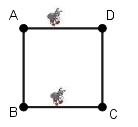
\includegraphics[scale=3.5]{Provas e Avaliações/arq-01.png}
\end{center}
Qual dos gráficos abaixo descreve a distância (em centímetros) entre as duas formiguinhas em função do tempo (em segundos)?
\begin{tasks}[counter-format={(tsk[a])},label-width=3.6ex, label-format = {\bfseries}, column-sep = {20pt}](2)
\task[\textcolor{blue}{$\negrito{(a)} $}] 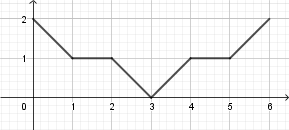
\includegraphics[scale=2.9]{Provas e Avaliações/arq-02.png}
\task[\textcolor{blue}{$\negrito{(b)} $}] 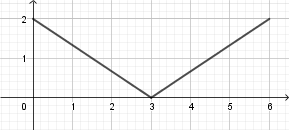
\includegraphics[scale=2.9]{Provas e Avaliações/arq-03.png}
\task[\textcolor{blue}{$\negrito{(c)} $}] 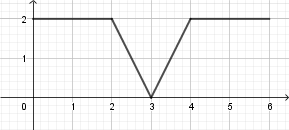
\includegraphics[scale=2.9]{Provas e Avaliações/arq-04.png}
\task[\textcolor{blue}{$\negrito{(d)} $}] 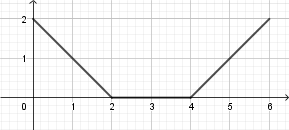
\includegraphics[scale=2.9]{Provas e Avaliações/arq-05.png}
\task[\textcolor{blue}{$\negrito{(e)} $}] 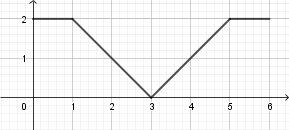
\includegraphics[scale=2.9]{Provas e Avaliações/arq-06.png}
\end{tasks}
\end{sol}
\textcolor{blue}{\textbf{Solução:}
As figuras abaixo mostram as posições relativas das formiguinhas em diferentes intervalos de tempo de $0$ s a $6$ s.}\newline
\begin{center}
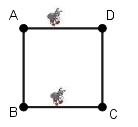
\includegraphics[scale=2.9]{Provas e Avaliações/arq-01 (1).png}
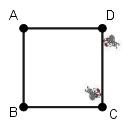
\includegraphics[scale=2.9]{Provas e Avaliações/arq-02 (1).png}
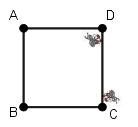
\includegraphics[scale=2.9]{Provas e Avaliações/arq-03 (1).png}
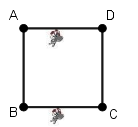
\includegraphics[scale=2.9]{Provas e Avaliações/arq-04 (1).png}
\end{center}
\textcolor{blue}{
\begin{itemize}
    \item Na primeira figura, observamos que de $0$ s a $2$ s, a distância entre as formiguinhas é constante e igual a $2$ cm.
    \item Na segunda figura, vemos que as formiguinhas andam uma em direção à outra e que a distância entre elas decresce a $2$ cm/s até ser $0$ cm no ponto médio de $CD$. Isso acontece entre os instantes $2$ s e $3$ s.
    \item  Na terceira figura, as formiguinhas começam a se distanciar e a distância entre elas cresce a $2$ cm/s até ser igual a $2$ cm. Isso acontece entre os instantes $3$ s e $4$ s.
    \item Na quarta figura, elas percorrem os segmentos de reta opostos mantendo a distância constante de $2$ cm entre os instantes $4$ s e $6$ s.
\end{itemize}
\begin{center}
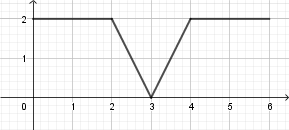
\includegraphics[scale=2.9]{Provas e Avaliações/arq-05 (1).png}
\end{center}
Logo, o gráfico que melhor representa a distância entre as duas formigas em função do tempo é o da alternativa (c).
}
\newpage
	\begin{sol}
\textit{(0,5 ponto)} \newline \newline A participação dos vendedores nos lucros de uma concessionária é diretamente proporcional às suas vendas. Os vendedores A, B e C venderam juntos $R\$\, 500.000,00$ em carros: A vendeu $R\$\, 225.000,00$, B vendeu $R\$\, 175.000,00$ e C, o restante. Eles dividiram entre si, a título de participação nos lucros, o valor de $R\$\, 10.000,00$. Nessa situação, A, B e C receberam, respectivamente, na participação dos lucros:
\begin{tasks}[counter-format={(tsk[a])},label-width=3.6ex, label-format = {\bfseries}, column-sep = {20pt}](1)
\task[\textcolor{blue}{$\negrito{(a)} $}] $R\$\, 3.150,00$, $R\$\, 2.450,00$ e $R\$\, 4.400,00$
\task[\textcolor{blue}{$\negrito{(b)} $}] $R\$\, 3.600,00$, $R\$\, 2.800,00$ e $R\$\, 3.600,00$  
\task[\textcolor{blue}{$\negrito{(c)} $}]$R\$\, 4.050,00$, $R\$\, 3.150,00$ e $R\$\, 2.800,00$          
\task[\textcolor{blue}{$\negrito{(d)} $}] $R\$\, 4.500,00$, $R\$\, 3.500,00$ e $R\$\, 2.000,00$  
\task[\textcolor{blue}{$\negrito{(e)} $}] $R\$\, 4.950,00$, $R\$\, 3.850,00$ e $R\$\, 1.200,00$
\end{tasks}
\end{sol}
\solucao{Primeiro calculemos o que o vendedor C vendeu
\[500.000 - (225.000 + 175.000)=100.000.\]
Sejam $x$, $y$ e $z$ os valores que A, B e C receberam na participação dos lucros respectivamente, então
\[\frac{x}{225.000}=\frac{y}{175.000}=\frac{z}{100.000}=\frac{10.000}{500.000}\]
Daí segue que $x=\frac{225.000 \times 10.000}{500.000}=4.500$, $y=\frac{175.000 \times 10.000}{500.000}=3.500$ e $z=\frac{100.000 \times 10.000}{500.000}=2.000$. Logo a opção correta é (d).
}
\newpage
	\begin{sol}
\textit{(4 pontos)} \newline \newline
Escreva a expressão $x^6+x^4+x^2y^2+y^4-y^6$ como produto de três fatores.\\
\textsf{Dica:} Fatore separadamente $x^6-y^6$ e $x^4+x^2y^2+y^4.$
\end{sol}
\solucao{Primeiro agrupamos os termos elevados a sexta e coloca todos elevados ao quadrado:
\[(x^3)^2 - (y^3)^2 + [(x^2)^2 + (xy)^2 + (y^2)^2]\]
A partir disso calculamos a diferença de quadrados na 1ª parte equação $(x^3)^2 - (y^3)^2:$
\[(x^3 + y^3) \cdot (x^3 - y^3) + [(x^2)^2 + (xy)^2 + (y^2)^2]\]
Assim, resolvemos a soma e a diferença de cubos $(x^3 + y^3)$ e $(x^3 - y^3):$\[(x+y) (x^2 - xy + y^2) \cdot (x-y) (x^2 + xy + y^2) + [(x^2)^2 + (xy)^2 + (y^2)^2]\]
Desenvolvendo mais um pouco:\[(x^2 - y^2) \cdot (x^2 + xy + y^2)(x^2 - xy + y^2) + [(x^2)^2 + (xy)^2 + (y^2)^2]\] 
Agora, fatorando a 2ª parte obtemos $ [(x^2)^2 + (xy)^2 + (y^2)^2]: $
\[[(x^2)^2 + (xy)^2 + (y^2)^2] = (x^2 + xy +y^2)(x^2 - xy +y^2)\]
Finalmente, nossa equação fica:\[(x^2 - y^2) \cdot (x^2 + xy + y^2)(x^2 - xy + y^2) + [(x^2 + xy +y^2)(x^2 - xy +y^2)]\]
Isolando o termo $(x^2 + xy +y^2)(x^2 - xy +y^2)$, temos:\[(x^2 + xy +y^2)(x^2 - xy +y^2) \cdot [(x^2 - y^2) +1]\]
Organizando a equação e tirando os colchetes obtemos:\[(x^2 + xy +y^2) (x^2 - xy +y^2)(x^2 - y^2 +1)\]
Portanto, concluímos que
\[\boxed{x^6+x^4+x^2y^2+y^4-y^6 = (x^2 + xy +y^2) (x^2 - xy +y^2) (x^2 - y^2 +1)}\]}
\begin{mdframed}
\textbf{Critérios de Correção:} \\
\begin{itemize}
    \item Fatorou $x^6 - y^6$ como $(x^3-y^3)(x^3+y^3)$: 0,5 pts;
    \item Fatorou $x^3 - y^3$ como $(x-y)(x^2 + xy + y^2)$: 1,0 pts;
    \item Fatorou $x^3 + y^3$ como $(x+y)(x^2 - xy + y^2)$: 1,0 pts;
    \item Fatorou $x^4 + x^2y^2 + y^4$ como $(x^2 + xy + y^2)(x^2 - xy + y^2)$: 1,0 pts;
    \item Chegou à fatoração final: 0,5 pts.
    \end{itemize}
    \end{mdframed}
\newpage
	\begin{sol}
\textit{(4 pontos)} \newline \newline
Em uma livraria, todos os livros são vendidos pelo preço unitário de $R\$\, 50,00$. O custo de produção é de $ R\$\, 10,00$ por livro e os gastos de manutenção da livraria com luz, água, telefone, funcionário e outros é de $R\$\, 2000,00$ por mês. Assim, por exemplo, se a livraria vende $200$ livros em um determinado mês, ela ganha $200 \times R\$\, 50,00=R\$\,10000,00$ e gasta $200 \times R\$\,10,00 = R\$\, 2000,00$ na produção dos livros, além de gastar $R\$\, 2000,00$ com manutenção, obtendo um lucro de $R\$\, 6000,00$ nesse mês.

\begin{tasks}[counter-format={(tsk[a])},label-width=3.6ex, label-format = {\bfseries}, column-sep = {20pt}](1)
\task[\textcolor{blue}{$\negrito{(a)} $}] Encontre uma expressão para o lucro mensal $L(x)$ em função do número $x$ de livros vendidos.
\task[\textcolor{blue}{$\negrito{(b)} $}] Qual é o menor  número de livros que devem ser vendidos em um determinado mês para a livraria não ter prejuízo naquele mês? (A livraria tem prejuízo quando $L(x)<0$)
\task[\textcolor{blue}{$\negrito{(c)} $}] O dono da livraria sente-se satisfeito em um determinado mês se ele obtiver um lucro de pelo menos $R\$\, 10000,00$ naquele mês. Para que o dono da livraria se sinta satisfeito em um determinado mês, qual é o menor número de livros que devem ser vendidos naquele mês?
\end{tasks}
\end{sol}
\solucao{\begin{tasks}[counter-format={(tsk[a])},label-width=3.6ex, label-format = {\bfseries}, column-sep = {20pt}](1)
\task[\textcolor{blue}{$\negrito{(a)} $}] A manutenção fixa por mês é de $R\$\, 2000,00$. A cada livro vendido, o lucro é de $R\$\, 50,00 - R\$\, 10,00 = R\$\, 40,00$. Dessa forma, o lucro da livraria por $x$ livros vendidos é de $L(x)=40x-2000$.
\task[\textcolor{blue}{$\negrito{(b)} $}] Para não ter prejuízo, o lucro não deve ser negativo, $L(x)=40x-2000 \geq 0$, isto é, $40x \geq 2000$. Dividindo por $40$ obtemos $x \geq 50$. Assim, o mínimo número de livros que devem ser vendidos em um determinado mês para a livraria não ter prejuízo é de $50$ livros naquele mês.
\task[\textcolor{blue}{$\negrito{(c)} $}] Para o dono se sentir satisfeito devemos ter $40x-2000 \geq 10000$. Somando $2000$ à inequação e dividindo por $40$, obtemos $x \geq 300$. Assim, o dono da livraria se sentirá satisfeito em um determinado mês se a livraria vender pelo menos $300$ livros naquele mês.
\end{tasks}}
\newpage
	\textcolor{Floresta}{\section{Avaliação Online}}
	\begin{sol}
\textit{(5 pontos)} \newline \newline	
	Alberto, Bernardo e Carlos disputaram uma corrida, em que cada um deles correu com velocidade constante durante todo o percurso. Eles largaram ao mesmo tempo na linha de partida. Quando Alberto cruzou a linha de chegada, Bernardo e Carlos estavam $36$ e $46$ metros atrás dele, respectivamente. Quando Bernardo cruzou a linha de chegada, Carlos estava $16$ metros atrás dele.
	\begin{tasks}[counter-format={(tsk[a])},label-width=3.6ex, label-format = {\bfseries}, column-sep = {20pt}](1)
\task[\textcolor{blue}{$\negrito{(a)} $}] Calcule a razão $\dfrac{v_B}{v_C}$, sendo $v_B$ e $v_C$ as velocidades de Bernardo e Carlos, respectivamente.
\task[\textcolor{blue}{$\negrito{(b)} $}] Qual é comprimento da pista?
\end{tasks}
\end{sol}
\solucao{	\begin{tasks}[counter-format={(tsk[a])},label-width=3.6ex, label-format = {\bfseries}, column-sep = {20pt}](1)
\task[\textcolor{blue}{$\negrito{(a)} $}] Quando Alberto cruzou a linha de chegada, a distância entre Bernardo e Carlos era de $10$ metros, e era $16$ metros quando Bernardo cruzou a linha de chegada. Assim, durante o tempo $t_1$ decorrido entre Alberto cruzar a linha de chegada e Bernardo cruzar a linha de chegada, Bernardo correu $36$ metros, enquanto Carlos correu $46-16=30$ metros. Assim, $v_B=\dfrac{36}{t_1}$  e $v_C=\dfrac{30}{t_1}$. Logo, $\dfrac{v_B}{v_C} =\dfrac{\frac{36}{t_1}}{\frac{30}{t_1}}=\dfrac{36}{30}=\dfrac{6}{5}$.
\task[\textcolor{blue}{$\negrito{(b)} $}] Seja $x$ o comprimento em metros da pista. Como Bernardo cruzou a linha de chegada $16$ metros à frente de Carlos, então $v_B=\dfrac{x}{t_2}$  e $v_C=\dfrac{x-16}{t_2}$ , sendo $t_2$ o tempo gasto para Bernardo percorrer a pista de corrida. Assim, $\dfrac{v_B}{v_C}=\dfrac{\frac{x}{t_2}}{\frac{x-16}{t_2}}=\dfrac{x}{x-16}$. Como $\dfrac{v_B}{v_C}=\dfrac{x}{x-16}$ e, pelo item (a), $\dfrac{v_B}{v_C}=\dfrac{6}{5}$, então $\dfrac{x}{x-16}=\dfrac{6}{5}$, ou seja, $6(x-16)=5x$. Resolvendo essa equação linear, obtém-se $x=96$.
\end{tasks}}
\begin{mdframed}
\textbf{Critérios de Correção:} \\
\begin{itemize}
    \item Atribuir $2,0$ pontos se o aluno calcular corretamente $\dfrac{v_B}{v_C}$. 
    \item Atribuir $2,0$ pontos se o aluno obtiver a equação $\dfrac{x}{x-16}=\dfrac{6}{5}$.
    \item Atribuir $1,0$ ponto se o aluno calcular corretamente o valor de $x$.
\end{itemize}
\end{mdframed}
\newpage
	\begin{sol}
\textit{(5 pontos)} \newline \newline
Considere a função afim $f(x)$ cujo gráfico passa pelo ponto $(8,3)$ e intersecta os eixos coordenados nos pontos $(\alpha,0)$ e $(0,-\beta-1)$, onde $\alpha$ e $\beta$ são números reais positivos. Determine a expressão de $f(x)$ sabendo que $\alpha\beta=8$.
\end{sol}
\solucao{Seja $f(x)=ax+b$ a expressão da função afim $f(x)$. Como o gráfico da função passa por $(0,-\beta-1)$, $(\alpha,0)$ e $(8,3)$, obtemos as relações $b=-\beta-1$, $\beta+1=a\alpha$ e $3=8a-\beta-1$ (ou ainda, $4=8a-\beta$). Multiplicando essa última equação por $\alpha$, temos $4\alpha=8a\alpha-\alpha\beta$. Substituindo $a\alpha=\beta+1$ e a relação dada no enunciado $\alpha\beta=8$, temos $4\alpha=8\beta$, ou seja, $\alpha=2\beta$. Como $\alpha\beta=8$, temos $\alpha^2=16$ e $\beta^2=4$. Como $\alpha$ e $\beta$ são positivos, então $\alpha=4$ e $\beta=2$. Logo, $a=\dfrac{3}{4}$ e $b=-3$, sendo, portanto, $f(x)=\dfrac{3}{4}x-3$.}
\begin{mdframed}
\textbf{Critérios de Correção:} \\
\begin{itemize}
    \item  Atribuir $1,0$ ponto se o aluno escrever, na forma de equação, as $3$ relações iniciais dadas pela pertinência dos pontos dados ao gráfico da função afim.
    \item   Atribuir $2,0$ pontos se o aluno obtiver uma das equações $\alpha^2=16$ ou $\beta^2=4$.
    \item  Atribuir $1,0$ ponto se o aluno utilizar o fato que $\alpha$ e $\beta$ são positivos para concluir que $\alpha=4$ e $\beta=2$.
    \item Atribuir $1,0$ ponto se o aluno encontrar a expressão da função afim.
\end{itemize}
\end{mdframed}
		%\vspace{60pt}
%		\newpage
		%QUESTAO 2
		
		%\vspace{60pt}
	
		%QUESTAO 3

		%\vspace{60pt}
		
		%QUESTAO 4 (OBJETIVA)

		
		%a)(  ) Alternativa A.
		
	%	b)(  ) Alternativa B.
		
	%	c)(  ) Alternativa C.
		
	%	d)(  ) Alternativa D.
		
	\flushbottom
	\flushright
%	"Alguma frase bonita de fim de prova"\\(autor da frase bonita)
\end{document}
\begin{center}
\includegraphics[scale=0.48]{paralelepipedo_p1}
\end{center}
	\begin{sol}
\textit{(4 pontos)} \newline \newline
\end{sol}
\solucao{}
\newpage